\section{Auswertung}
\label{sec:Auswertung}

\subsection{Lange Spule}

Im folgenden wird die magnetische Flussdichte einer langen Spule gemessen und graphisch dargestellt.
%\begin{minipage}{0.5\textwidth}
\begin{table}
\centering
\caption{Messdaten der langen Spule}
\begin{tabular}{c c}
  \toprule
  x (m) &  B (10e-3 T) \\
  \midrule
  -0.02 &         0.23 \\
  -0.01 &         0.28 \\
  -0.01 &         0.35 \\
  -0.01 &         0.46 \\
    0.00 &         0.60 \\
    0.01 &         0.84 \\
    0.01 &         1.15 \\
    0.01 &         1.43 \\
    0.02 &         1.70 \\
    0.03 &         1.89 \\
    0.03 &         2.02 \\
    0.04 &         2.12 \\
    0.04 &         2.18 \\
  \bottomrule
\end{tabular}
\end{table}
%\end{minipage}

%\begin{minipage}{0.5\textwidth}
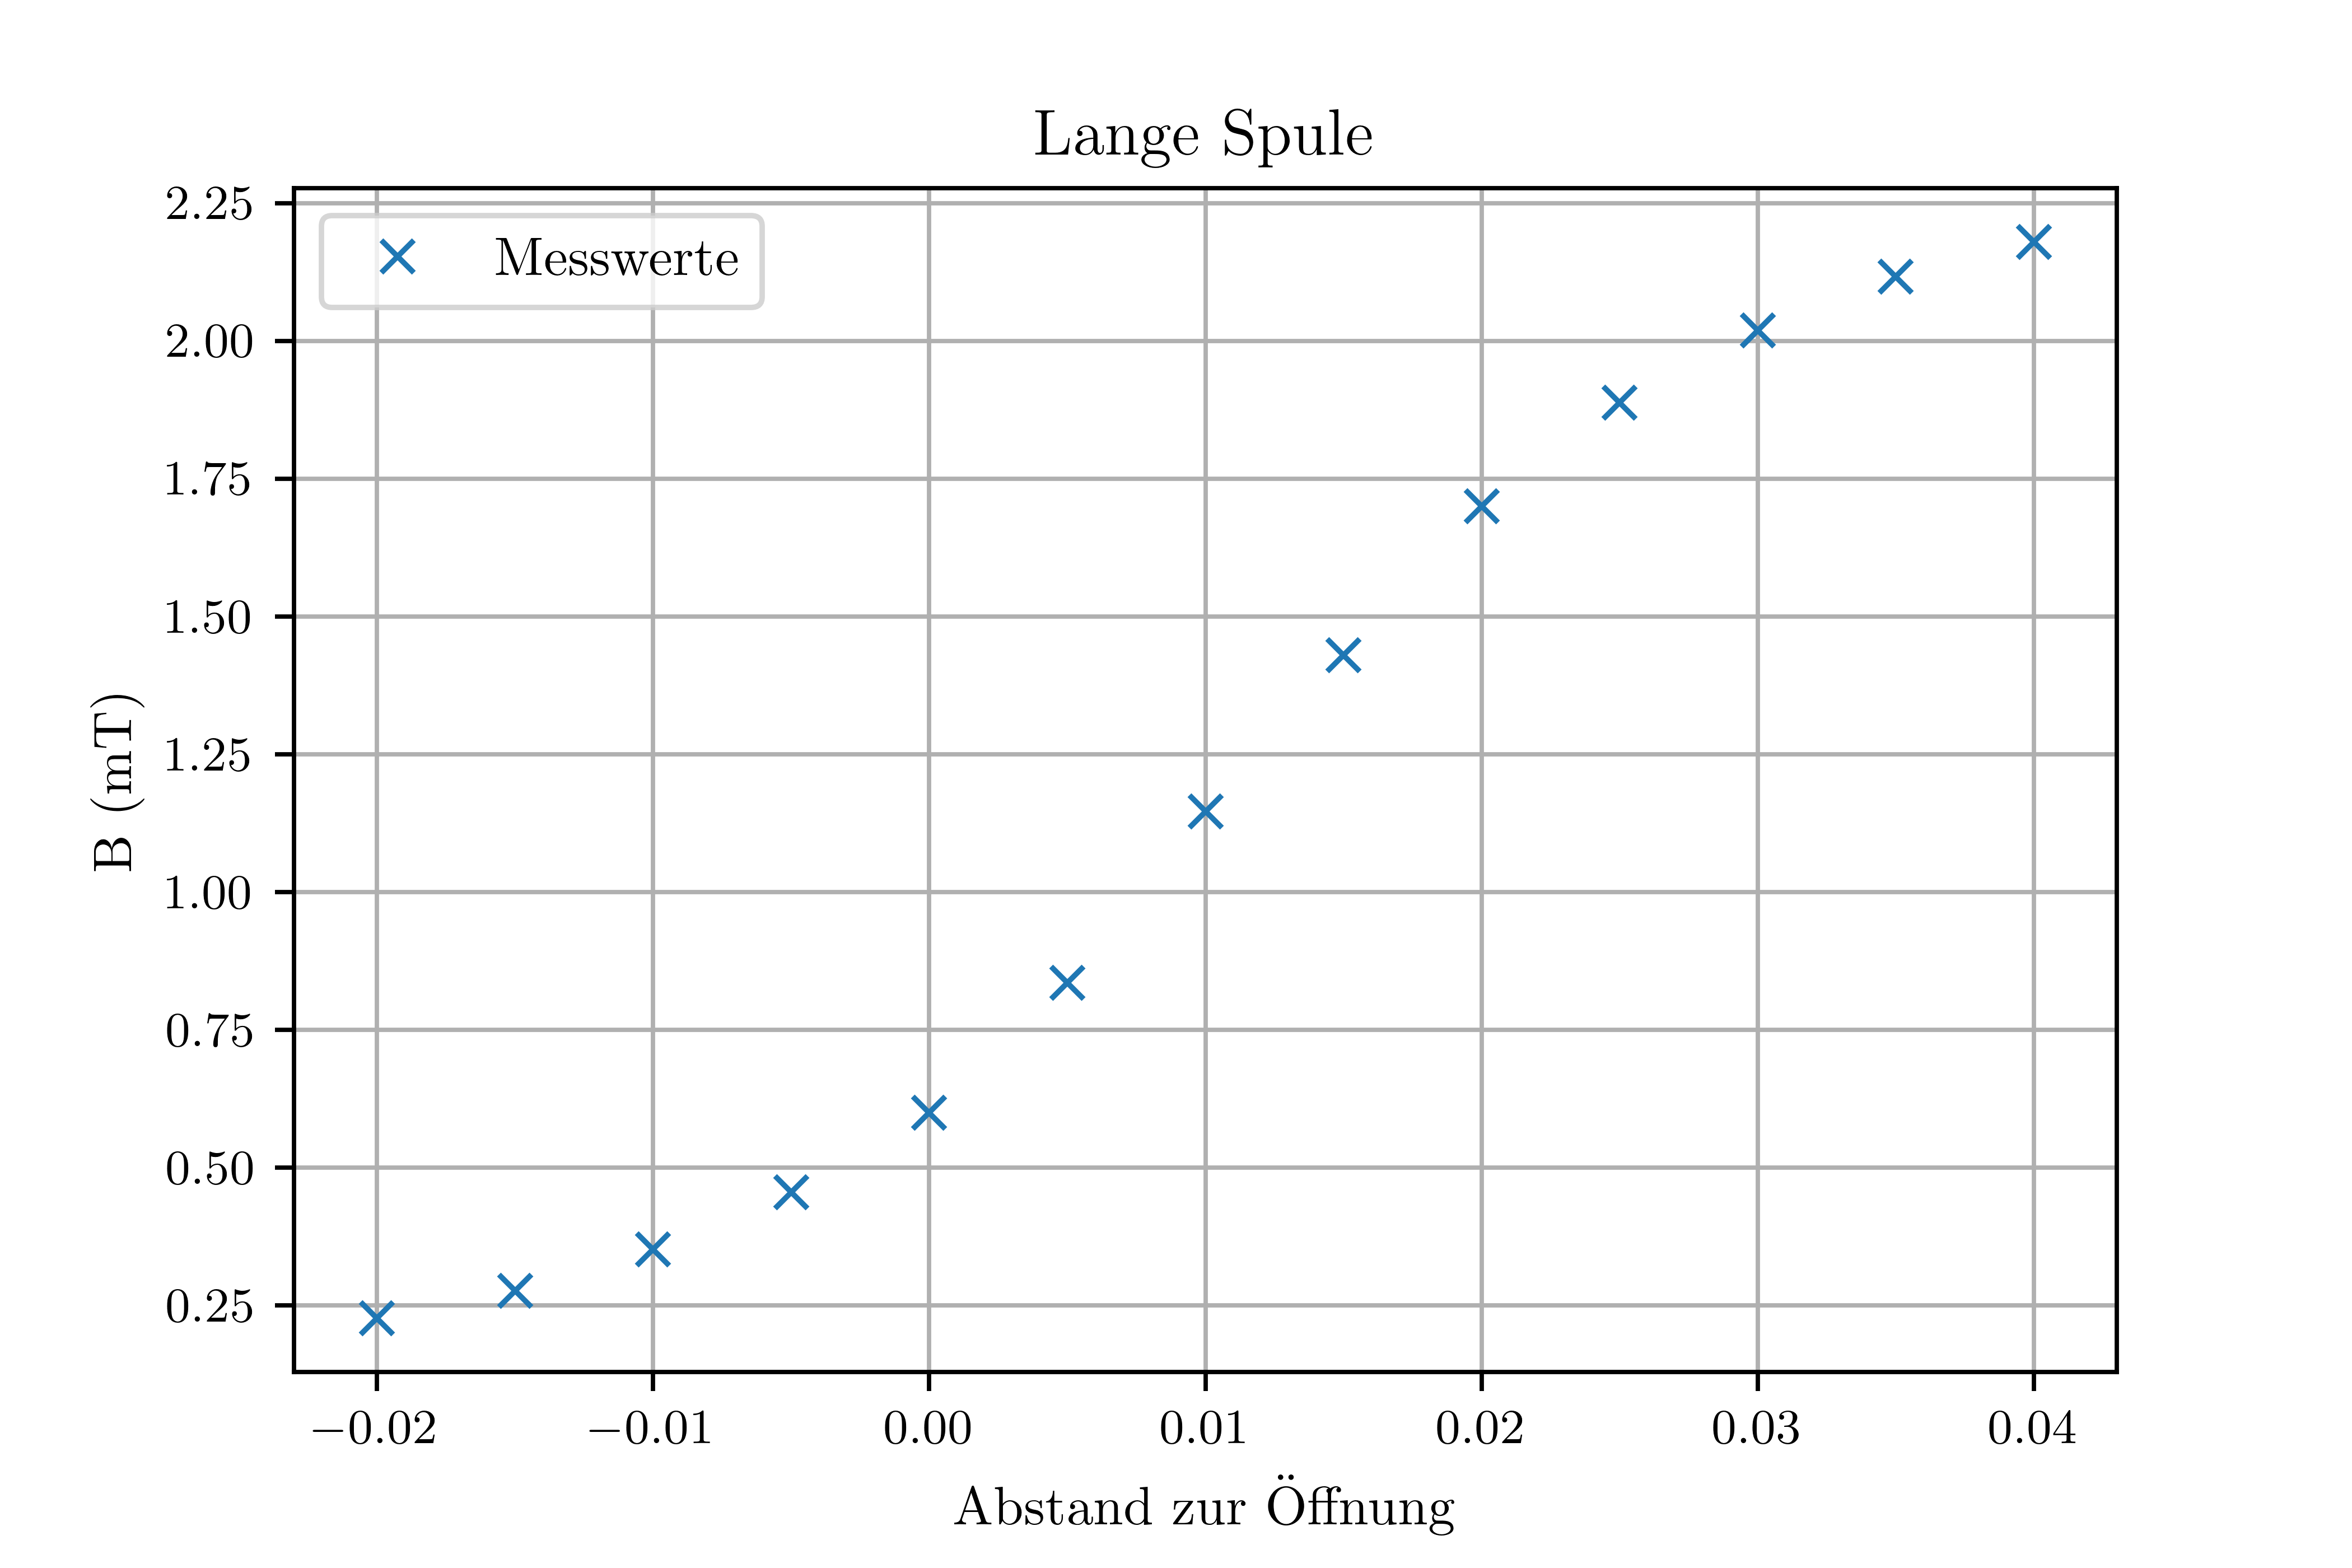
\includegraphics[width=\textwidth]{pictures/LangeSpule1.png}    %Hier fehlt noch die Beschriftung
%\end{minipage}

Es ist eine abflachende Steigung des Magnetfeldes zu erkennen. Der Theoriewert, der sich aus der Formel (\ref{eq:LangeSpule}) ergibt, lautet:
\begin{equation}
  B_{\text{LS}} = 2.31 T
\end{equation}


\subsection{Helmholtzspulenpaar}

Im folgenden sind die Messdaten für die Abstände $d_{1} = 0.012m$, $d_{1} = 0.014m$ und $d_{1} = 0.016m$ in Tabellen und Plots dargestellt.

